\documentclass[a4paper,9pt]{extarticle}

% --- PACKAGES ESSENTIELS ---
\usepackage[utf8]{inputenc}
\usepackage[T1]{fontenc}
\usepackage{helvet}
\renewcommand{\familydefault}{\sfdefault}

\usepackage[left=0.8cm, right=0.8cm, top=0.65cm, bottom=0.65cm]{geometry}
\usepackage{xcolor}
\usepackage{titlesec}
\usepackage{enumitem}
\usepackage{tabularx}
\usepackage{fontawesome5}
\usepackage[hidelinks]{hyperref}
\usepackage{tikz}

\pagestyle{empty}

% --- COULEURS PROFESSIONNELLES & MODERNES ---
\definecolor{primary}{HTML}{0F172A}      % Slate / Bleu Marine Profond (#0F172A)
\definecolor{accent}{HTML}{2563EB}       % Bleu Royal Électrique (#2563EB)
\definecolor{accentteal}{HTML}{0D9488}   % Sarcelle / IA & Data Highlight (#0D9488)
\definecolor{textdark}{HTML}{1E293B}     % Texte principal très lisible
\definecolor{textmuted}{HTML}{475569}    % Métadonnées / Dates / Lieux
\definecolor{linegray}{HTML}{CBD5E1}     % Séparateurs discrets
\definecolor{tagbg}{HTML}{F8FAFC}        % Arrière-plan badges
\definecolor{tagborder}{HTML}{CBD5E1}    % Bordure badges

% --- CONFIGURATION DES LIENS ---
\hypersetup{
    colorlinks=true,
    urlcolor=accent,
    linkcolor=accent
}

% Supprimer les warnings hyperref pour les glyphes FontAwesome
\pdfstringdefDisableCommands{%
  \def\faUser{}%
  \def\faBriefcase{}%
  \def\faCogs{}%
  \def\faGraduationCap{}%
  \def\faCubes{}%
  \def\faAward{}%
  \def\faLanguage{}%
  \def\faHeart{}%
  \def\faExternalLink*{}%
  \def\faCalendar*{}%
}

% --- FORMAT DES TITRES DE SECTION ---
\titleformat{\section}
  {\color{primary}\bfseries\small}
  {}{0em}
  {}[\vspace{-2.5pt}{\color{accent}\rule{\linewidth}{1.1pt}}\vspace{-2pt}]

\titlespacing{\section}{0pt}{3.5pt}{2pt}

% --- LISTES COMPACTES ---
\setlist[itemize]{
  noitemsep,
  topsep=1pt,
  parsep=0pt,
  partopsep=0pt,
  leftmargin=9pt,
  label={\color{accent}\scriptsize\faAngleRight}
}

% --- MACROS PERSONNALISÉES ---
\newcommand{\cvhighlight}[1]{\textcolor{accentteal}{\textbf{#1}}}
\newcommand{\cvtech}[1]{\textcolor{primary}{\textbf{#1}}}

\newcommand{\cvtag}[1]{%
  \tikz[baseline=-0.5ex]\node[draw=tagborder, fill=tagbg, rounded corners=2pt, inner xsep=3pt, inner ysep=1pt, font=\fontsize{6.5pt}{7.5pt}\selectfont\sffamily\color{primary}]{#1};%
}

\setlength{\parindent}{0pt}
\setlength{\parskip}{0pt}

\begin{document}

%=============================================================================
% EN-TÊTE DU CV AVEC PHOTO (HEADER)
%=============================================================================
\noindent
\begin{tabularx}{\linewidth}{@{} X r @{}}
  \begin{minipage}[c]{0.82\linewidth}
    {\LARGE \textbf{\color{primary} ASSIA NOUAOURY}}\\[2.5pt]
    {\small \textbf{\color{accent} ÉLÈVE-INGÉNIEUR EN 5\textsuperscript{ÈME} ANNÉE -- IA, BIG DATA \& DATA ENGINEERING}}\\[2.5pt]
    {\footnotesize \color{textmuted} À la recherche d'un \textbf{\color{primary}Stage PFE (Projet de Fin d'Études)} en Data Engineering, IA ou Développement Logiciel | 2026}\\[4pt]
    {\footnotesize \color{textdark}
      \faEnvelope\ \href{mailto:assianouaoury@gmail.com}{assianouaoury@gmail.com} \quad\textbar\quad
      \faPhone*\ +212 620-433358 \quad\textbar\quad
      \faMapMarker*\ Casablanca, Maroc
    }
  \end{minipage}
  &
  \begin{tikzpicture}[baseline=(current bounding box.center)]
    \clip (0,0) circle (1.15cm);
    \node at (0,0) {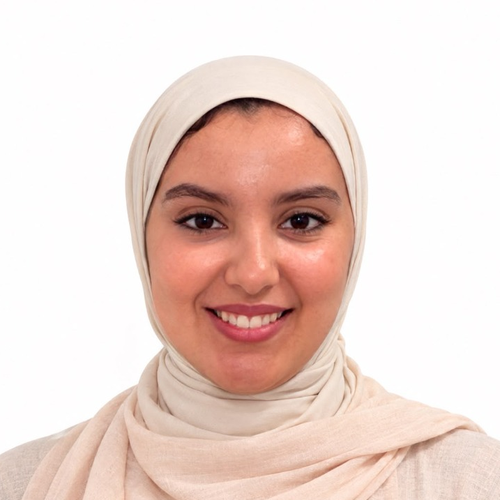
\includegraphics[width=2.35cm]{assia_photo.png}};
    \draw[line width=1.5pt, color=accent] (0,0) circle (1.15cm);
  \end{tikzpicture}
\end{tabularx}

\vspace{1pt}
\noindent{\color{linegray}\rule{\linewidth}{0.8pt}}
\vspace{2pt}

%=============================================================================
% CORPS DU CV : MISE EN PAGE 2 COLONNES (57.5% GAUCHE / 40.5% DROITE)
%=============================================================================
\noindent
\begin{minipage}[t]{0.575\textwidth}

  %----------- PROFIL -----------
  \section{\faUser\ Profil Professionnel}
  {\footnotesize \color{textdark}
  Élève-Ingénieur en 5\textsuperscript{ème} année à l'\textbf{EMSI}, spécialisée en \cvhighlight{IA, Data Science \& Data Engineering}. Passionnée par la conception de \cvtech{pipelines de données (ETL/ELT)}, le streaming temps réel avec \cvtech{Apache Kafka} et l'intégration de \cvtech{modèles d'IA avancés (LangGraph/LLMs)}. Forte de stages et projets concrets, je recherche un stage PFE pour concevoir des architectures data et applicatives innovantes à fort impact.
  }

  \vspace{2.5pt}

  %----------- EXPÉRIENCES -----------
  \section{\faBriefcase\ Expériences Professionnelles}

  % DELTA TOURS
  \textbf{\color{primary} Stagiaire Développeuse Full-Stack \& IA} \hfill {\scriptsize\color{textmuted}\faCalendar*\ 07/2025 -- 09/2025}\\
  {\footnotesize \textbf{\color{accent} DELTA TOURS}} \hfill {\scriptsize\color{textmuted}\faMapMarker*\ Casablanca, Maroc}
  \begin{itemize}
    \item Conception et développement d'une plateforme web complète de réservation touristique.
    \item Développement des modules front-end (\cvtech{React / Vite}) et de l'API REST sous \cvtech{FastAPI}.
    \item Modélisation relationnelle, gestion des offres et sécurisation des accès avec \cvtech{JWT}.
    \item Intégration d'un assistant intelligent basé sur \cvhighlight{LangGraph \& Ollama} pour répondre en langage naturel sur les offres, circuits et tarifs.
  \end{itemize}
  \vspace{1.5pt}
  {\scriptsize \textbf{\color{textmuted}Technologies :}\ \cvtag{React} \cvtag{FastAPI} \cvtag{LangGraph} \cvtag{Ollama} \cvtag{SQLAlchemy} \cvtag{PostgreSQL}}

  \vspace{3.5pt}

  % TYM SOLUTIONS
  \textbf{\color{primary} Stagiaire Développeuse Web} \hfill {\scriptsize\color{textmuted}\faCalendar*\ 06/2025 -- 08/2025}\\
  {\footnotesize \textbf{\color{accent} TYM SOLUTIONS}} \hfill {\scriptsize\color{textmuted}\faMapMarker*\ Casablanca, Maroc}
  \begin{itemize}
    \item Participation au développement de la plateforme e-santé \cvhighlight{Sahtek}.
    \item Développement d'interfaces web réactives, ergonomiques et modernes avec \cvtech{Vue.js}.
    \item Optimisation du parcours utilisateur et intégration responsive.
  \end{itemize}
  \vspace{1.5pt}
  {\scriptsize \textbf{\color{textmuted}Technologies :}\ \cvtag{Vue.js} \cvtag{JavaScript} \cvtag{HTML5} \cvtag{CSS3} \cvtag{E-Santé}}

  \vspace{2.5pt}

  %----------- PROJETS RÉALISÉS -----------
  \section{\faCogs\ Projets d'Ingénierie \& PFA}

  % FILM-A & STREAMING
  \textbf{\color{primary} Plateforme de Recommandation \& Streaming -- Film-A} \hfill {\scriptsize\color{textmuted}\faCalendar*\ 2025 -- 2026}\\
  {\scriptsize\color{textmuted} Pipeline ETL, Streaming Kafka \& Graphes Neo4j}
  \begin{itemize}
    \item Pipeline \cvhighlight{ETL} automatisé pour l'extraction, nettoyage et indexation de données vers \cvhighlight{Neo4j}.
    \item Ingestion continue des flux d'événements et interactions utilisateurs en temps réel via \cvtech{Apache Kafka}.
    \item Moteur de recommandation basé sur les relations de graphes et assistant IA.
    \item Backend sous \cvtech{Node.js / Python} avec APIs REST et application mobile sous \cvtech{React Native}.
  \end{itemize}
  \vspace{1.5pt}
  {\scriptsize \textbf{\color{textmuted}Technologies :}\ \cvtag{Apache Kafka} \cvtag{ETL} \cvtag{Neo4j} \cvtag{Python} \cvtag{React Native} \cvtag{Node.js}}

  \vspace{3.5pt}

  % ODYSSEY PFA
  \textbf{\color{primary} Plateforme de Réservation de Voyages -- Odyssey (PFA)} \hfill {\scriptsize\color{textmuted}\faCalendar*\ 2025 -- 2026}\\
  {\scriptsize\color{textmuted} Architecture 3-tiers \& Recommandation Intelligente}
  \begin{itemize}
    \item Plateforme web dynamique de réservation basée sur la saisonnalité des destinations.
    \item Conception d'une \cvhighlight{architecture 3-tiers} avec gestion des réservations et transactions.
    \item Intégration d'un assistant conversationnel IA et d'un module de géolocalisation GPS.
    \item Gestion des rôles utilisateurs et interface d'administration sécurisée.
  \end{itemize}
  \vspace{1.5pt}
  {\scriptsize \textbf{\color{textmuted}Technologies :}\ \cvtag{C\#} \cvtag{ASP.NET Core} \cvtag{Razor Pages} \cvtag{SQL Server} \cvtag{IA}}

  \vspace{3.5pt}

  % PIPELINE STREAMING & ETL
  \textbf{\color{primary} Pipeline de Données Distribué \& Traitement ETL} \hfill {\scriptsize\color{textmuted}\faCalendar*\ 2024 -- 2025}\\
  {\scriptsize\color{textmuted} Architecture Événementielle, Ingestion Multi-Sources \& Analytics}
  \begin{itemize}
    \item Architecture de streaming orientée événements avec \cvhighlight{Apache Kafka} pour l'ingestion de flux continus.
    \item Pipelines \cvhighlight{ETL / ELT} sous \cvtech{Python (Pandas / SQL)} pour le nettoyage et l'agrégation de données.
    \item Stockage relationnel sous \cvtech{PostgreSQL} et conteneurisation des services avec \cvtech{Docker}.
  \end{itemize}
  \vspace{1.5pt}
  {\scriptsize \textbf{\color{textmuted}Technologies :}\ \cvtag{Apache Kafka} \cvtag{ETL/ELT} \cvtag{Python} \cvtag{PostgreSQL} \cvtag{Docker}}

\end{minipage}
\hfill
%=============================================================================
% COLONNE DE DROITE (SIDEBAR : 40.5% DE LARGEUR, POLICES VISIBLES & LISIBLES)
%=============================================================================
\begin{minipage}[t]{0.405\textwidth}

  %----------- FORMATION -----------
  \section{\faGraduationCap\ Formation}

  \textbf{\color{primary}\small Cycle Ingénieur d'État} \hfill {\scriptsize\color{textmuted}\faCalendar*\ 2022 -- 2026}\\
  {\small \textbf{EMSI Casablanca}}\\
  {\footnotesize École Marocaine des Sciences de l'Ingénieur}\\
  {\footnotesize Filière : \cvhighlight{Informatique et Réseaux}}\\
  {\footnotesize Option : \textbf{Intelligence Artificielle \& Data Science}}\\
  {\scriptsize\textit{5\textsuperscript{ème} année (Dernière année -- PFE 2026)}}

  \vspace{3pt}

  \textbf{\color{primary}\small Baccalauréat Scientifique} \hfill {\scriptsize\color{textmuted}\faCalendar*\ 2021 -- 2022}\\
  {\small \textbf{Lycée Manar Al Khair}}\\
  {\footnotesize Sciences Physiques et Chimie}

  \vspace{3pt}

  %----------- COMPÉTENCES -----------
  \section{\faCubes\ Compétences Clés}

  {\footnotesize \textbf{\color{accent} Data Engineering \& Streaming}}
  \begin{itemize}
    \item Pipelines \textbf{ETL / ELT}, \textbf{Apache Kafka} (Streaming)
    \item Ingestion continue, Flux temps réel, Data Quality
    \item Traitement de données (\textbf{Pandas}, \textbf{PySpark}, \textbf{SQL})
  \end{itemize}

  \vspace{2pt}
  {\footnotesize \textbf{\color{accent} Intelligence Artificielle \& Machine Learning}}
  \begin{itemize}
    \item LLMs, LangGraph, Ollama, Chatbots, IA Générative
    \item Moteurs de Recommandation, Graphes (\textbf{Neo4j})
    \item Python, Scikit-learn, Algorithmes prédictifs
  \end{itemize}

  \vspace{2pt}
  {\footnotesize \textbf{\color{accent} Développement Back-End \& Architecture}}
  \begin{itemize}
    \item FastAPI, ASP.NET Core (C\#), Node.js, Django
    \item Architecture 3-tiers \& Événementielle, APIs REST
  \end{itemize}

  \vspace{2pt}
  {\footnotesize \textbf{\color{accent} Front-End, BDD \& Outils DevOps}}
  \begin{itemize}
    \item React, React Native, Vue.js, TypeScript
    \item PostgreSQL, SQL Server, MySQL, SQLite
    \item Docker, Git, Linux, Firebase
  \end{itemize}

  \vspace{3pt}

  %----------- CERTIFICATIONS -----------
  \section{\faAward\ Certifications Clés}

  \textbf{\color{primary}\small Software Engineering} \hfill {\scriptsize\color{textmuted} 2025}\\
  {\footnotesize \textbf{Coursera / Spécialisation}}\\
  {\scriptsize\color{textdark} Architecture Logicielle, SDLC, Méthodologies}

  \vspace{2.5pt}
  \textbf{\color{primary}\small Using Python to Access Web Data} \hfill {\scriptsize\color{textmuted} 2025}\\
  {\footnotesize \textbf{University of Michigan}}\\
  {\scriptsize\color{textdark} Ingestion de Données, Web Scraping, REST APIs}

  \vspace{2.5pt}
  \textbf{\color{primary}\small React Native} \hfill {\scriptsize\color{textmuted} 2025}\\
  {\footnotesize \textbf{Meta}}\\
  {\scriptsize\color{textdark} Développement Mobile Multiplateforme \& UI}

  \vspace{2.5pt}
  \textbf{\color{primary}\small Interactivity with JavaScript} \hfill {\scriptsize\color{textmuted} 2025}\\
  {\footnotesize \textbf{University of Michigan}}\\
  {\scriptsize\color{textdark} DOM Manipulation, Événements, UI Dynamique}

  \vspace{2.5pt}
  \textbf{\color{primary}\small Programmation Orientée Objet en C++} \hfill {\scriptsize\color{textmuted} 2025}\\
  {\footnotesize \textbf{EPFL}}\\
  {\scriptsize\color{textdark} Gestion Mémoire, Algorithmes \& Complexité}

  \vspace{2.5pt}
  \textbf{\color{primary}\small Successful Negotiation \& Presentation} \hfill {\scriptsize\color{textmuted} 2024}\\
  {\footnotesize \textbf{University of Michigan}}\\
  {\scriptsize\color{textdark} Communication Professionnelle \& Négociation}

  \vspace{3pt}

  %----------- LANGUES -----------
  \section{\faLanguage\ Langues}
  {\footnotesize
    \textbf{Arabe :} Langue maternelle\\[1pt]
    \textbf{Français :} Courant (C1 / Professionnel)\\[1pt]
    \textbf{Anglais :} Courant (B2/C1 / Technique)
  }

  \vspace{3pt}

  %----------- ATOUTS & INTÉRÊTS -----------
  \section{\faHeart\ Centres d'Intérêt}
  {\footnotesize
    \faRobot\ Veille technologique en IA \& LLMs\\[1pt]
    \faCode\ Développement Web \& Mobile créatif\\[1pt]
    \faUsers\ Travail en équipe \& Projets collaboratifs
  }

\end{minipage}

\end{document}
